\documentclass[twoside]{book}

% Packages required by doxygen
\usepackage{fixltx2e}
\usepackage{calc}
\usepackage{doxygen}
\usepackage[export]{adjustbox} % also loads graphicx
\usepackage{graphicx}
\usepackage[utf8]{inputenc}
\usepackage{makeidx}
\usepackage{multicol}
\usepackage{multirow}
\PassOptionsToPackage{warn}{textcomp}
\usepackage{textcomp}
\usepackage[nointegrals]{wasysym}
\usepackage[table]{xcolor}

% Font selection
\usepackage[T1]{fontenc}
\usepackage[scaled=.90]{helvet}
\usepackage{courier}
\usepackage{amssymb}
\usepackage{sectsty}
\renewcommand{\familydefault}{\sfdefault}
\allsectionsfont{%
  \fontseries{bc}\selectfont%
  \color{darkgray}%
}
\renewcommand{\DoxyLabelFont}{%
  \fontseries{bc}\selectfont%
  \color{darkgray}%
}
\newcommand{\+}{\discretionary{\mbox{\scriptsize$\hookleftarrow$}}{}{}}

% Page & text layout
\usepackage{geometry}
\geometry{%
  a4paper,%
  top=2.5cm,%
  bottom=2.5cm,%
  left=2.5cm,%
  right=2.5cm%
}
\tolerance=750
\hfuzz=15pt
\hbadness=750
\setlength{\emergencystretch}{15pt}
\setlength{\parindent}{0cm}
\setlength{\parskip}{3ex plus 2ex minus 2ex}
\makeatletter
\renewcommand{\paragraph}{%
  \@startsection{paragraph}{4}{0ex}{-1.0ex}{1.0ex}{%
    \normalfont\normalsize\bfseries\SS@parafont%
  }%
}
\renewcommand{\subparagraph}{%
  \@startsection{subparagraph}{5}{0ex}{-1.0ex}{1.0ex}{%
    \normalfont\normalsize\bfseries\SS@subparafont%
  }%
}
\makeatother

% Headers & footers
\usepackage{fancyhdr}
\pagestyle{fancyplain}
\fancyhead[LE]{\fancyplain{}{\bfseries\thepage}}
\fancyhead[CE]{\fancyplain{}{}}
\fancyhead[RE]{\fancyplain{}{\bfseries\leftmark}}
\fancyhead[LO]{\fancyplain{}{\bfseries\rightmark}}
\fancyhead[CO]{\fancyplain{}{}}
\fancyhead[RO]{\fancyplain{}{\bfseries\thepage}}
\fancyfoot[LE]{\fancyplain{}{}}
\fancyfoot[CE]{\fancyplain{}{}}
\fancyfoot[RE]{\fancyplain{}{\bfseries\scriptsize Generated by Doxygen }}
\fancyfoot[LO]{\fancyplain{}{\bfseries\scriptsize Generated by Doxygen }}
\fancyfoot[CO]{\fancyplain{}{}}
\fancyfoot[RO]{\fancyplain{}{}}
\renewcommand{\footrulewidth}{0.4pt}
\renewcommand{\chaptermark}[1]{%
  \markboth{#1}{}%
}
\renewcommand{\sectionmark}[1]{%
  \markright{\thesection\ #1}%
}

% Indices & bibliography
\usepackage{natbib}
\usepackage[titles]{tocloft}
\setcounter{tocdepth}{3}
\setcounter{secnumdepth}{5}
\makeindex

% Hyperlinks (required, but should be loaded last)
\usepackage{ifpdf}
\ifpdf
  \usepackage[pdftex,pagebackref=true]{hyperref}
\else
  \usepackage[ps2pdf,pagebackref=true]{hyperref}
\fi
\hypersetup{%
  colorlinks=true,%
  linkcolor=blue,%
  citecolor=blue,%
  unicode%
}

% Custom commands
\newcommand{\clearemptydoublepage}{%
  \newpage{\pagestyle{empty}\cleardoublepage}%
}

\usepackage{caption}
\captionsetup{labelsep=space,justification=centering,font={bf},singlelinecheck=off,skip=4pt,position=top}

%===== C O N T E N T S =====

\begin{document}

% Titlepage & ToC
\hypersetup{pageanchor=false,
             bookmarksnumbered=true,
             pdfencoding=unicode
            }
\pagenumbering{alph}
\begin{titlepage}
\vspace*{7cm}
\begin{center}%
{\Large Chronotrigger \\[1ex]\large V1.\+0.\+0 }\\
\vspace*{1cm}
{\large Generated by Doxygen 1.8.14}\\
\end{center}
\end{titlepage}
\clearemptydoublepage
\pagenumbering{roman}
\tableofcontents
\clearemptydoublepage
\pagenumbering{arabic}
\hypersetup{pageanchor=true}

%--- Begin generated contents ---
\chapter{Have the camera a certain rect with Crono in the middle}
\label{md_docs_Notes}
\Hypertarget{md_docs_Notes}

\begin{DoxyItemize}
\item if the image is smaller than the camera then it doesn\textquotesingle{}t move
\end{DoxyItemize}

\section*{class \hyperlink{classBackground}{Background} needs to include the width and height of the viewable bg}


\begin{DoxyItemize}
\item Is this a good solution?
\begin{DoxyItemize}
\item use the overlay/collision grid for each bg instead have a set w/h for it and if the camera hits the edge of that it should stop
\item Gonna need to have positions for that anyway might as well use it\textquotesingle{}s edges for the map collision
\end{DoxyItemize}
\item This is necessary for determining whether the camera is larger than the image?
\item Necessary if the bg changes in some way
\begin{DoxyItemize}
\item E.\+g. Crono\textquotesingle{}s house when his mom opens window 
\end{DoxyItemize}
\end{DoxyItemize}
\chapter{Scope}
\label{md_README}
\Hypertarget{md_README}
For right now all I want to do is make Crono\textquotesingle{}s house. Possibly more to follow afterwards, but initially I just want to do that.

\subsection*{Collission detection}


\begin{DoxyItemize}
\item Walls
\item Objects
\item Characters -\/ only if we do more than just Crono\textquotesingle{}s room
\begin{DoxyItemize}
\item Special case here as we should be able to walk through a character after pushing for so long
\item doorways -\/ same character
\end{DoxyItemize}
\end{DoxyItemize}

\subsection*{Sprites}


\begin{DoxyItemize}
\item Furniture in Crono\textquotesingle{}s room
\item Backgrounds
\begin{DoxyItemize}
\item Are these included in the background or separate objects?
\end{DoxyItemize}
\item Cat -\/ must have since it\textquotesingle{}s there when crono wakes up
\item Mother -\/ She wakes him up
\item The man himself
\end{DoxyItemize}

\subsection*{Cutscene}


\begin{DoxyItemize}
\item Mother waking crono up \subsection*{Text}
\end{DoxyItemize}


\begin{DoxyItemize}
\item Mother waking crono up
\item Lucca convo in the kitchen -\/ if we decide to do more than just Crono\textquotesingle{}s room
\end{DoxyItemize}

\subsection*{Loading zones}


\begin{DoxyItemize}
\item If we do the first floor of the house
\end{DoxyItemize}

\subsection*{character customization, naming, identification}


\begin{DoxyItemize}
\item When mother asks for Lucca\textquotesingle{}s name
\begin{DoxyItemize}
\item Default name of Lucca
\item Can change that once and only once
\end{DoxyItemize}
\end{DoxyItemize}

\subsection*{\hyperlink{classCharacter}{Character} portrait images}


\begin{DoxyItemize}
\item Only playable characters now
\end{DoxyItemize}

\subsection*{Triangle menu}


\begin{DoxyItemize}
\item All submenus
\begin{DoxyItemize}
\item Items
\item \hyperlink{classCharacter}{Character} stats
\item Saving
\begin{DoxyItemize}
\item this doesn\textquotesingle{}t need to work right now
\end{DoxyItemize}
\item config
\begin{DoxyItemize}
\item Include screen size in that among other things
\end{DoxyItemize}
\end{DoxyItemize}
\end{DoxyItemize}

...

So much more to come holy crap 
\chapter{Hierarchical Index}
\section{Class Hierarchy}
This inheritance list is sorted roughly, but not completely, alphabetically\+:\begin{DoxyCompactList}
\item \contentsline{section}{Character}{\pageref{classCharacter}}{}
\item \contentsline{section}{Constants}{\pageref{classConstants}}{}
\begin{DoxyCompactList}
\item \contentsline{section}{Background}{\pageref{classBackground}}{}
\end{DoxyCompactList}
\item \contentsline{section}{Sprite\+Sheet}{\pageref{classSpriteSheet}}{}
\end{DoxyCompactList}

\chapter{Class Index}
\section{Class List}
Here are the classes, structs, unions and interfaces with brief descriptions\+:\begin{DoxyCompactList}
\item\contentsline{section}{\hyperlink{classBackground}{Background} }{\pageref{classBackground}}{}
\item\contentsline{section}{\hyperlink{classCharacter}{Character} }{\pageref{classCharacter}}{}
\item\contentsline{section}{\hyperlink{classConstants}{Constants} }{\pageref{classConstants}}{}
\item\contentsline{section}{\hyperlink{classSpriteSheet}{Sprite\+Sheet} }{\pageref{classSpriteSheet}}{}
\end{DoxyCompactList}

\chapter{File Index}
\section{File List}
Here is a list of all files with brief descriptions\+:\begin{DoxyCompactList}
\item\contentsline{section}{\hyperlink{main_8cpp}{main.\+cpp} }{\pageref{main_8cpp}}{}
\item\contentsline{section}{include/\hyperlink{config_8h}{config.\+h} }{\pageref{config_8h}}{}
\item\contentsline{section}{include/\hyperlink{SpriteSheet_8h}{Sprite\+Sheet.\+h} }{\pageref{SpriteSheet_8h}}{}
\item\contentsline{section}{include/classes/\hyperlink{Background_8h}{Background.\+h} }{\pageref{Background_8h}}{}
\item\contentsline{section}{include/classes/\hyperlink{Character_8h}{Character.\+h} }{\pageref{Character_8h}}{}
\item\contentsline{section}{include/classes/\hyperlink{PlayableCharacter_8h}{Playable\+Character.\+h} }{\pageref{PlayableCharacter_8h}}{}
\item\contentsline{section}{include/classes/\hyperlink{classes_2SpriteSheet_8h}{Sprite\+Sheet.\+h} }{\pageref{classes_2SpriteSheet_8h}}{}
\item\contentsline{section}{include/utilities/\hyperlink{utilities_2config_8h}{config.\+h} }{\pageref{utilities_2config_8h}}{}
\item\contentsline{section}{include/utilities/\hyperlink{Constants_8h}{Constants.\+h} }{\pageref{Constants_8h}}{}
\item\contentsline{section}{include/utilities/\hyperlink{DestroySdlObjects_8h}{Destroy\+Sdl\+Objects.\+h} }{\pageref{DestroySdlObjects_8h}}{}
\item\contentsline{section}{include/utilities/\hyperlink{errorHandlers_8h}{error\+Handlers.\+h} }{\pageref{errorHandlers_8h}}{}
\item\contentsline{section}{include/utilities/\hyperlink{utilities_8h}{utilities.\+h} }{\pageref{utilities_8h}}{}
\item\contentsline{section}{src/classes/\hyperlink{Background_8cpp}{Background.\+cpp} }{\pageref{Background_8cpp}}{}
\item\contentsline{section}{src/utilities/\hyperlink{Constants_8cpp}{Constants.\+cpp} }{\pageref{Constants_8cpp}}{}
\item\contentsline{section}{src/utilities/\hyperlink{errorHandlers_8cpp}{error\+Handlers.\+cpp} }{\pageref{errorHandlers_8cpp}}{}
\item\contentsline{section}{src/utilities/\hyperlink{utilities_8cpp}{utilities.\+cpp} }{\pageref{utilities_8cpp}}{}
\end{DoxyCompactList}

\chapter{Class Documentation}
\hypertarget{classBackground}{}\section{Background Class Reference}
\label{classBackground}\index{Background@{Background}}


{\ttfamily \#include $<$Background.\+h$>$}

Inheritance diagram for Background\+:\begin{figure}[H]
\begin{center}
\leavevmode
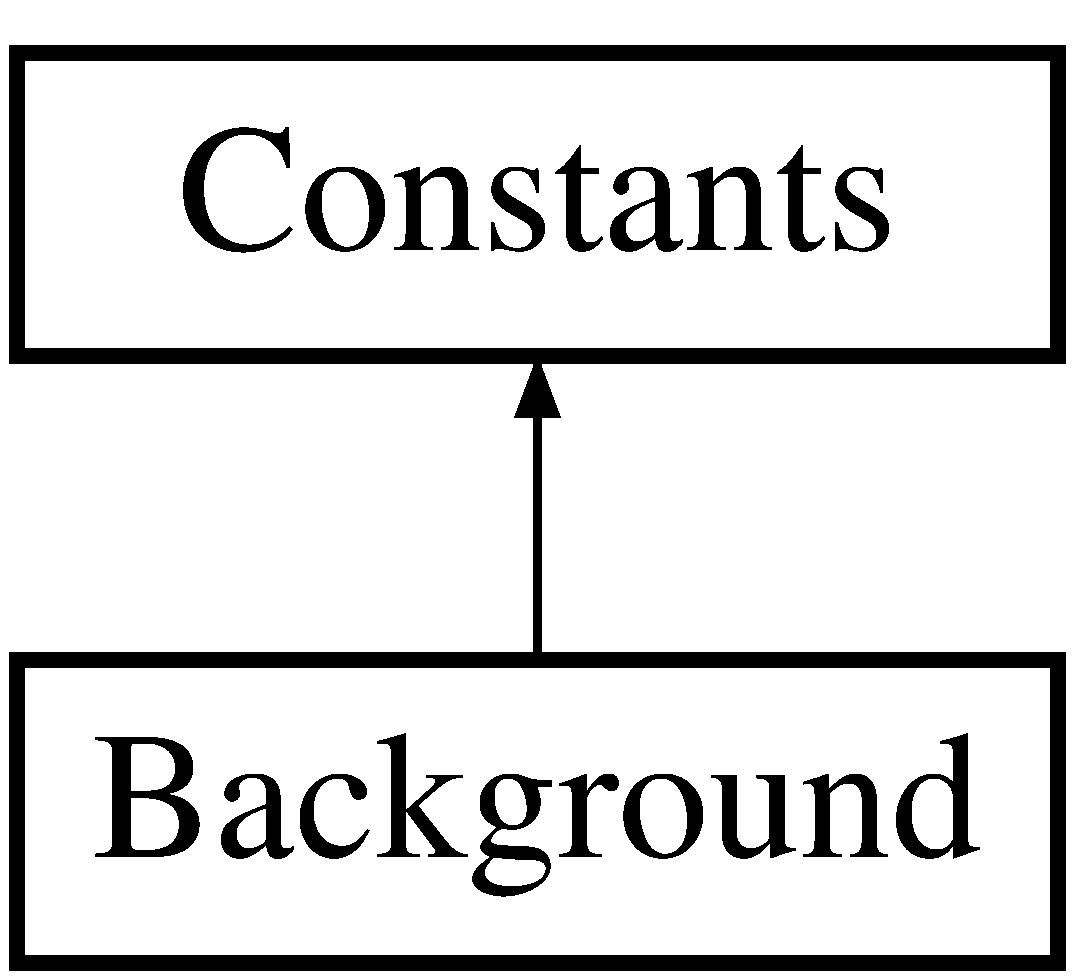
\includegraphics[height=2.000000cm]{classBackground}
\end{center}
\end{figure}
\subsection*{Public Member Functions}
\begin{DoxyCompactItemize}
\item 
\hyperlink{classBackground_a05b686e4ce0cbdb3b1fa14a93fdf98a1}{Background} ()
\item 
\hyperlink{classBackground_a40a6b9d526e79ddf5fc2d0201f17b540}{Background} (std\+::string new\+B\+G\+File)
\item 
\hyperlink{classBackground_aedede892eac3a2e2b9a2bf6191e80217}{Background} (std\+::string new\+B\+G\+File, S\+D\+L\+\_\+\+Renderer $\ast$new\+Ren, S\+D\+L\+\_\+\+Window $\ast$new\+Win)
\item 
std\+::string \hyperlink{classBackground_af76fb5926c3c73dc82090795e094252d}{get\+B\+G\+File} ()
\item 
S\+D\+L\+\_\+\+Texture $\ast$ \hyperlink{classBackground_ad155a21be25b01e6dfc4d5aa3592570e}{get\+B\+G\+Texture} ()
\item 
bool \hyperlink{classBackground_ad2d7cd387529a4257802dcb4235ff3ff}{set\+B\+G\+Texture} (S\+D\+L\+\_\+\+Renderer $\ast$ren, S\+D\+L\+\_\+\+Window $\ast$win)
\item 
void \hyperlink{classBackground_a52f039c01025184caaab3886dc591be6}{set\+B\+G\+File} (std\+::string new\+B\+G\+File)
\end{DoxyCompactItemize}


\subsection{Detailed Description}
This class contains the background/image data. E.\+g. Chrono\textquotesingle{}s house, Leene square, etc. 

\subsection{Constructor \& Destructor Documentation}
\mbox{\Hypertarget{classBackground_a05b686e4ce0cbdb3b1fa14a93fdf98a1}\label{classBackground_a05b686e4ce0cbdb3b1fa14a93fdf98a1}} 
\index{Background@{Background}!Background@{Background}}
\index{Background@{Background}!Background@{Background}}
\subsubsection{\texorpdfstring{Background()}{Background()}\hspace{0.1cm}{\footnotesize\ttfamily [1/3]}}
{\footnotesize\ttfamily Background\+::\+Background (\begin{DoxyParamCaption}{ }\end{DoxyParamCaption})}

\mbox{\Hypertarget{classBackground_a40a6b9d526e79ddf5fc2d0201f17b540}\label{classBackground_a40a6b9d526e79ddf5fc2d0201f17b540}} 
\index{Background@{Background}!Background@{Background}}
\index{Background@{Background}!Background@{Background}}
\subsubsection{\texorpdfstring{Background()}{Background()}\hspace{0.1cm}{\footnotesize\ttfamily [2/3]}}
{\footnotesize\ttfamily Background\+::\+Background (\begin{DoxyParamCaption}\item[{std\+::string}]{new\+B\+G\+File }\end{DoxyParamCaption})}

\mbox{\Hypertarget{classBackground_aedede892eac3a2e2b9a2bf6191e80217}\label{classBackground_aedede892eac3a2e2b9a2bf6191e80217}} 
\index{Background@{Background}!Background@{Background}}
\index{Background@{Background}!Background@{Background}}
\subsubsection{\texorpdfstring{Background()}{Background()}\hspace{0.1cm}{\footnotesize\ttfamily [3/3]}}
{\footnotesize\ttfamily Background\+::\+Background (\begin{DoxyParamCaption}\item[{std\+::string}]{new\+B\+G\+File,  }\item[{S\+D\+L\+\_\+\+Renderer $\ast$}]{new\+Ren,  }\item[{S\+D\+L\+\_\+\+Window $\ast$}]{new\+Win }\end{DoxyParamCaption})}



\subsection{Member Function Documentation}
\mbox{\Hypertarget{classBackground_af76fb5926c3c73dc82090795e094252d}\label{classBackground_af76fb5926c3c73dc82090795e094252d}} 
\index{Background@{Background}!get\+B\+G\+File@{get\+B\+G\+File}}
\index{get\+B\+G\+File@{get\+B\+G\+File}!Background@{Background}}
\subsubsection{\texorpdfstring{get\+B\+G\+File()}{getBGFile()}}
{\footnotesize\ttfamily std\+::string Background\+::get\+B\+G\+File (\begin{DoxyParamCaption}{ }\end{DoxyParamCaption})}

\mbox{\Hypertarget{classBackground_ad155a21be25b01e6dfc4d5aa3592570e}\label{classBackground_ad155a21be25b01e6dfc4d5aa3592570e}} 
\index{Background@{Background}!get\+B\+G\+Texture@{get\+B\+G\+Texture}}
\index{get\+B\+G\+Texture@{get\+B\+G\+Texture}!Background@{Background}}
\subsubsection{\texorpdfstring{get\+B\+G\+Texture()}{getBGTexture()}}
{\footnotesize\ttfamily S\+D\+L\+\_\+\+Texture $\ast$ Background\+::get\+B\+G\+Texture (\begin{DoxyParamCaption}{ }\end{DoxyParamCaption})}

\mbox{\Hypertarget{classBackground_a52f039c01025184caaab3886dc591be6}\label{classBackground_a52f039c01025184caaab3886dc591be6}} 
\index{Background@{Background}!set\+B\+G\+File@{set\+B\+G\+File}}
\index{set\+B\+G\+File@{set\+B\+G\+File}!Background@{Background}}
\subsubsection{\texorpdfstring{set\+B\+G\+File()}{setBGFile()}}
{\footnotesize\ttfamily void Background\+::set\+B\+G\+File (\begin{DoxyParamCaption}\item[{std\+::string}]{new\+B\+G\+File }\end{DoxyParamCaption})}

\mbox{\Hypertarget{classBackground_ad2d7cd387529a4257802dcb4235ff3ff}\label{classBackground_ad2d7cd387529a4257802dcb4235ff3ff}} 
\index{Background@{Background}!set\+B\+G\+Texture@{set\+B\+G\+Texture}}
\index{set\+B\+G\+Texture@{set\+B\+G\+Texture}!Background@{Background}}
\subsubsection{\texorpdfstring{set\+B\+G\+Texture()}{setBGTexture()}}
{\footnotesize\ttfamily bool Background\+::set\+B\+G\+Texture (\begin{DoxyParamCaption}\item[{S\+D\+L\+\_\+\+Renderer $\ast$}]{ren,  }\item[{S\+D\+L\+\_\+\+Window $\ast$}]{win }\end{DoxyParamCaption})}



The documentation for this class was generated from the following files\+:\begin{DoxyCompactItemize}
\item 
include/classes/\hyperlink{Background_8h}{Background.\+h}\item 
src/classes/\hyperlink{Background_8cpp}{Background.\+cpp}\end{DoxyCompactItemize}

\hypertarget{classCharacter}{}\section{Character Class Reference}
\label{classCharacter}\index{Character@{Character}}


{\ttfamily \#include $<$Character.\+h$>$}



The documentation for this class was generated from the following file\+:\begin{DoxyCompactItemize}
\item 
include/classes/\hyperlink{Character_8h}{Character.\+h}\end{DoxyCompactItemize}

\hypertarget{classConstants}{}\section{Constants Class Reference}
\label{classConstants}\index{Constants@{Constants}}


{\ttfamily \#include $<$Constants.\+h$>$}

Inheritance diagram for Constants\+:\begin{figure}[H]
\begin{center}
\leavevmode
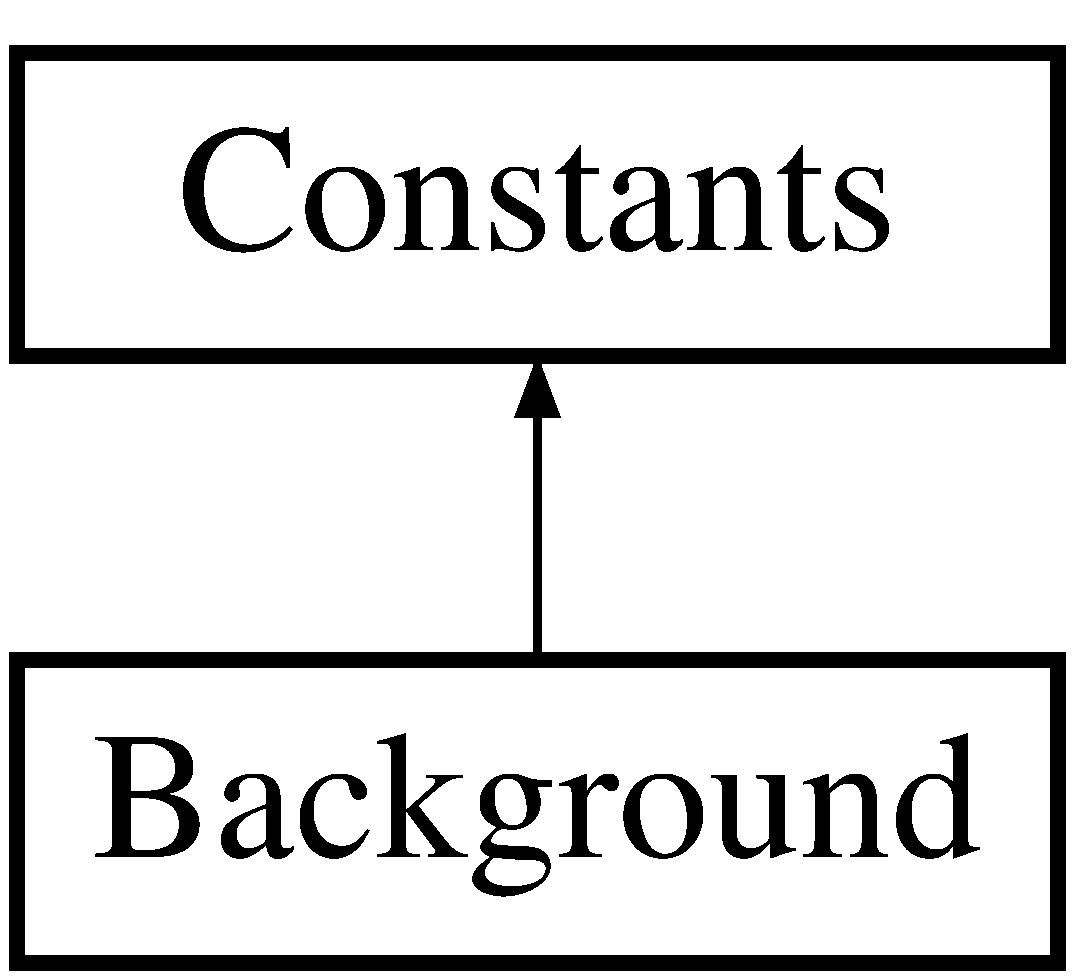
\includegraphics[height=2.000000cm]{classConstants}
\end{center}
\end{figure}
\subsection*{Public Member Functions}
\begin{DoxyCompactItemize}
\item 
string \hyperlink{classConstants_a192570c7395cc199c295be25c851ab59}{get\+B\+G\+Path} ()
\item 
string \hyperlink{classConstants_a2017e0f60d08822215e0876e50e7a671}{get\+Error\+Message} (int idx)
\item 
int \hyperlink{classConstants_a99ee472396cb27f43e1c17541e9cd071}{get\+Camera\+Width} ()
\item 
int \hyperlink{classConstants_a04a1764de8928d2fca5cf2555735a405}{get\+Camera\+Height} ()
\end{DoxyCompactItemize}


\subsection{Detailed Description}
These constants are used only by the program, there\textquotesingle{}s a separate config file for user specific options 

\subsection{Member Function Documentation}
\mbox{\Hypertarget{classConstants_a192570c7395cc199c295be25c851ab59}\label{classConstants_a192570c7395cc199c295be25c851ab59}} 
\index{Constants@{Constants}!get\+B\+G\+Path@{get\+B\+G\+Path}}
\index{get\+B\+G\+Path@{get\+B\+G\+Path}!Constants@{Constants}}
\subsubsection{\texorpdfstring{get\+B\+G\+Path()}{getBGPath()}}
{\footnotesize\ttfamily string Constants\+::get\+B\+G\+Path (\begin{DoxyParamCaption}{ }\end{DoxyParamCaption})}

\mbox{\Hypertarget{classConstants_a04a1764de8928d2fca5cf2555735a405}\label{classConstants_a04a1764de8928d2fca5cf2555735a405}} 
\index{Constants@{Constants}!get\+Camera\+Height@{get\+Camera\+Height}}
\index{get\+Camera\+Height@{get\+Camera\+Height}!Constants@{Constants}}
\subsubsection{\texorpdfstring{get\+Camera\+Height()}{getCameraHeight()}}
{\footnotesize\ttfamily int Constants\+::get\+Camera\+Height (\begin{DoxyParamCaption}{ }\end{DoxyParamCaption})}

\mbox{\Hypertarget{classConstants_a99ee472396cb27f43e1c17541e9cd071}\label{classConstants_a99ee472396cb27f43e1c17541e9cd071}} 
\index{Constants@{Constants}!get\+Camera\+Width@{get\+Camera\+Width}}
\index{get\+Camera\+Width@{get\+Camera\+Width}!Constants@{Constants}}
\subsubsection{\texorpdfstring{get\+Camera\+Width()}{getCameraWidth()}}
{\footnotesize\ttfamily int Constants\+::get\+Camera\+Width (\begin{DoxyParamCaption}{ }\end{DoxyParamCaption})}

\mbox{\Hypertarget{classConstants_a2017e0f60d08822215e0876e50e7a671}\label{classConstants_a2017e0f60d08822215e0876e50e7a671}} 
\index{Constants@{Constants}!get\+Error\+Message@{get\+Error\+Message}}
\index{get\+Error\+Message@{get\+Error\+Message}!Constants@{Constants}}
\subsubsection{\texorpdfstring{get\+Error\+Message()}{getErrorMessage()}}
{\footnotesize\ttfamily string Constants\+::get\+Error\+Message (\begin{DoxyParamCaption}\item[{int}]{idx }\end{DoxyParamCaption})}



The documentation for this class was generated from the following files\+:\begin{DoxyCompactItemize}
\item 
include/utilities/\hyperlink{Constants_8h}{Constants.\+h}\item 
src/utilities/\hyperlink{Constants_8cpp}{Constants.\+cpp}\end{DoxyCompactItemize}

\hypertarget{classSpriteSheet}{}\section{Sprite\+Sheet Class Reference}
\label{classSpriteSheet}\index{Sprite\+Sheet@{Sprite\+Sheet}}


{\ttfamily \#include $<$Sprite\+Sheet.\+h$>$}

\subsection*{Public Member Functions}
\begin{DoxyCompactItemize}
\item 
void \hyperlink{classSpriteSheet_ab635dd55f278dc207b00b709b951709f}{set\+Sheet\+Name} (string newsheet\+Name)
\item 
string \hyperlink{classSpriteSheet_ad06ca62e3dc2a880a6741e8dd26e6134}{get\+Sheet\+Name} ()
\item 
void \hyperlink{classSpriteSheet_ab635dd55f278dc207b00b709b951709f}{set\+Sheet\+Name} (string newsheet\+Name)
\item 
string \hyperlink{classSpriteSheet_ad06ca62e3dc2a880a6741e8dd26e6134}{get\+Sheet\+Name} ()
\end{DoxyCompactItemize}


\subsection{Member Function Documentation}
\mbox{\Hypertarget{classSpriteSheet_ad06ca62e3dc2a880a6741e8dd26e6134}\label{classSpriteSheet_ad06ca62e3dc2a880a6741e8dd26e6134}} 
\index{Sprite\+Sheet@{Sprite\+Sheet}!get\+Sheet\+Name@{get\+Sheet\+Name}}
\index{get\+Sheet\+Name@{get\+Sheet\+Name}!Sprite\+Sheet@{Sprite\+Sheet}}
\subsubsection{\texorpdfstring{get\+Sheet\+Name()}{getSheetName()}\hspace{0.1cm}{\footnotesize\ttfamily [1/2]}}
{\footnotesize\ttfamily string Sprite\+Sheet\+::get\+Sheet\+Name (\begin{DoxyParamCaption}{ }\end{DoxyParamCaption})}

\mbox{\Hypertarget{classSpriteSheet_ad06ca62e3dc2a880a6741e8dd26e6134}\label{classSpriteSheet_ad06ca62e3dc2a880a6741e8dd26e6134}} 
\index{Sprite\+Sheet@{Sprite\+Sheet}!get\+Sheet\+Name@{get\+Sheet\+Name}}
\index{get\+Sheet\+Name@{get\+Sheet\+Name}!Sprite\+Sheet@{Sprite\+Sheet}}
\subsubsection{\texorpdfstring{get\+Sheet\+Name()}{getSheetName()}\hspace{0.1cm}{\footnotesize\ttfamily [2/2]}}
{\footnotesize\ttfamily string Sprite\+Sheet\+::get\+Sheet\+Name (\begin{DoxyParamCaption}{ }\end{DoxyParamCaption})}

\mbox{\Hypertarget{classSpriteSheet_ab635dd55f278dc207b00b709b951709f}\label{classSpriteSheet_ab635dd55f278dc207b00b709b951709f}} 
\index{Sprite\+Sheet@{Sprite\+Sheet}!set\+Sheet\+Name@{set\+Sheet\+Name}}
\index{set\+Sheet\+Name@{set\+Sheet\+Name}!Sprite\+Sheet@{Sprite\+Sheet}}
\subsubsection{\texorpdfstring{set\+Sheet\+Name()}{setSheetName()}\hspace{0.1cm}{\footnotesize\ttfamily [1/2]}}
{\footnotesize\ttfamily void Sprite\+Sheet\+::set\+Sheet\+Name (\begin{DoxyParamCaption}\item[{string}]{newsheet\+Name }\end{DoxyParamCaption})}

\mbox{\Hypertarget{classSpriteSheet_ab635dd55f278dc207b00b709b951709f}\label{classSpriteSheet_ab635dd55f278dc207b00b709b951709f}} 
\index{Sprite\+Sheet@{Sprite\+Sheet}!set\+Sheet\+Name@{set\+Sheet\+Name}}
\index{set\+Sheet\+Name@{set\+Sheet\+Name}!Sprite\+Sheet@{Sprite\+Sheet}}
\subsubsection{\texorpdfstring{set\+Sheet\+Name()}{setSheetName()}\hspace{0.1cm}{\footnotesize\ttfamily [2/2]}}
{\footnotesize\ttfamily void Sprite\+Sheet\+::set\+Sheet\+Name (\begin{DoxyParamCaption}\item[{string}]{newsheet\+Name }\end{DoxyParamCaption})}



The documentation for this class was generated from the following file\+:\begin{DoxyCompactItemize}
\item 
include/classes/\hyperlink{classes_2SpriteSheet_8h}{Sprite\+Sheet.\+h}\end{DoxyCompactItemize}

\chapter{File Documentation}
\hypertarget{Notes_8md}{}\section{docs/\+Notes.md File Reference}
\label{Notes_8md}\index{docs/\+Notes.\+md@{docs/\+Notes.\+md}}

\hypertarget{Background_8h}{}\section{include/classes/\+Background.h File Reference}
\label{Background_8h}\index{include/classes/\+Background.\+h@{include/classes/\+Background.\+h}}
{\ttfamily \#include \char`\"{}Constants.\+h\char`\"{}}\newline
\subsection*{Classes}
\begin{DoxyCompactItemize}
\item 
class \hyperlink{classBackground}{Background}
\end{DoxyCompactItemize}

\hypertarget{Character_8h}{}\section{include/classes/\+Character.h File Reference}
\label{Character_8h}\index{include/classes/\+Character.\+h@{include/classes/\+Character.\+h}}
\subsection*{Classes}
\begin{DoxyCompactItemize}
\item 
class \hyperlink{classCharacter}{Character}
\end{DoxyCompactItemize}

\hypertarget{PlayableCharacter_8h}{}\section{include/classes/\+Playable\+Character.h File Reference}
\label{PlayableCharacter_8h}\index{include/classes/\+Playable\+Character.\+h@{include/classes/\+Playable\+Character.\+h}}

\hypertarget{classes_2SpriteSheet_8h}{}\section{include/classes/\+Sprite\+Sheet.h File Reference}
\label{classes_2SpriteSheet_8h}\index{include/classes/\+Sprite\+Sheet.\+h@{include/classes/\+Sprite\+Sheet.\+h}}
\subsection*{Classes}
\begin{DoxyCompactItemize}
\item 
class \hyperlink{classSpriteSheet}{Sprite\+Sheet}
\end{DoxyCompactItemize}

\hypertarget{SpriteSheet_8h}{}\section{include/\+Sprite\+Sheet.h File Reference}
\label{SpriteSheet_8h}\index{include/\+Sprite\+Sheet.\+h@{include/\+Sprite\+Sheet.\+h}}
\subsection*{Classes}
\begin{DoxyCompactItemize}
\item 
class \hyperlink{classSpriteSheet}{Sprite\+Sheet}
\end{DoxyCompactItemize}

\hypertarget{config_8h}{}\section{include/config.h File Reference}
\label{config_8h}\index{include/config.\+h@{include/config.\+h}}
{\ttfamily \#include $<$map$>$}\newline
{\ttfamily \#include $<$string$>$}\newline
\subsection*{Variables}
\begin{DoxyCompactItemize}
\item 
const map$<$ int, string $>$ \hyperlink{config_8h_a572c201077c60da3aeae64cf70195b2d}{error\+Messages}
\item 
const int \hyperlink{config_8h_ade92e07203a3ba6835aab188b841658f}{screen\+\_\+width} = 1024
\item 
const int \hyperlink{config_8h_a52afc0b1078a0ef9af887430f8e8b84c}{screen\+\_\+height} = 768
\item 
const int \hyperlink{config_8h_a1c45a0531f0e35db600a28df03a348c1}{tile\+\_\+size} = 40
\end{DoxyCompactItemize}


\subsection{Variable Documentation}
\mbox{\Hypertarget{config_8h_a572c201077c60da3aeae64cf70195b2d}\label{config_8h_a572c201077c60da3aeae64cf70195b2d}} 
\index{config.\+h@{config.\+h}!error\+Messages@{error\+Messages}}
\index{error\+Messages@{error\+Messages}!config.\+h@{config.\+h}}
\subsubsection{\texorpdfstring{error\+Messages}{errorMessages}}
{\footnotesize\ttfamily const map$<$int, string$>$ error\+Messages}

{\bfseries Initial value\+:}
\begin{DoxyCode}
= \{
    \{0, \textcolor{stringliteral}{"SDL Surface load error"}\},
    \{1, \textcolor{stringliteral}{"Could not create texture from surface"}\}
\}
\end{DoxyCode}
\mbox{\Hypertarget{config_8h_a52afc0b1078a0ef9af887430f8e8b84c}\label{config_8h_a52afc0b1078a0ef9af887430f8e8b84c}} 
\index{config.\+h@{config.\+h}!screen\+\_\+height@{screen\+\_\+height}}
\index{screen\+\_\+height@{screen\+\_\+height}!config.\+h@{config.\+h}}
\subsubsection{\texorpdfstring{screen\+\_\+height}{screen\_height}}
{\footnotesize\ttfamily const int screen\+\_\+height = 768}

\mbox{\Hypertarget{config_8h_ade92e07203a3ba6835aab188b841658f}\label{config_8h_ade92e07203a3ba6835aab188b841658f}} 
\index{config.\+h@{config.\+h}!screen\+\_\+width@{screen\+\_\+width}}
\index{screen\+\_\+width@{screen\+\_\+width}!config.\+h@{config.\+h}}
\subsubsection{\texorpdfstring{screen\+\_\+width}{screen\_width}}
{\footnotesize\ttfamily const int screen\+\_\+width = 1024}

\mbox{\Hypertarget{config_8h_a1c45a0531f0e35db600a28df03a348c1}\label{config_8h_a1c45a0531f0e35db600a28df03a348c1}} 
\index{config.\+h@{config.\+h}!tile\+\_\+size@{tile\+\_\+size}}
\index{tile\+\_\+size@{tile\+\_\+size}!config.\+h@{config.\+h}}
\subsubsection{\texorpdfstring{tile\+\_\+size}{tile\_size}}
{\footnotesize\ttfamily const int tile\+\_\+size = 40}


\hypertarget{utilities_2config_8h}{}\section{include/utilities/config.h File Reference}
\label{utilities_2config_8h}\index{include/utilities/config.\+h@{include/utilities/config.\+h}}
{\ttfamily \#include $<$map$>$}\newline
{\ttfamily \#include $<$string$>$}\newline
\subsection*{Variables}
\begin{DoxyCompactItemize}
\item 
const map$<$ int, string $>$ \hyperlink{utilities_2config_8h_a572c201077c60da3aeae64cf70195b2d}{error\+Messages}
\item 
string \hyperlink{utilities_2config_8h_a69f8564381dee22430c7dd0c3da80090}{resource\+Path} = \char`\"{}\char`\"{}
\item 
const int \hyperlink{utilities_2config_8h_ade92e07203a3ba6835aab188b841658f}{screen\+\_\+width} = 1024
\item 
const int \hyperlink{utilities_2config_8h_a52afc0b1078a0ef9af887430f8e8b84c}{screen\+\_\+height} = 768
\item 
const int \hyperlink{utilities_2config_8h_a1c45a0531f0e35db600a28df03a348c1}{tile\+\_\+size} = 40
\end{DoxyCompactItemize}


\subsection{Variable Documentation}
\mbox{\Hypertarget{utilities_2config_8h_a572c201077c60da3aeae64cf70195b2d}\label{utilities_2config_8h_a572c201077c60da3aeae64cf70195b2d}} 
\index{utilities/config.\+h@{utilities/config.\+h}!error\+Messages@{error\+Messages}}
\index{error\+Messages@{error\+Messages}!utilities/config.\+h@{utilities/config.\+h}}
\subsubsection{\texorpdfstring{error\+Messages}{errorMessages}}
{\footnotesize\ttfamily const map$<$int, string$>$ error\+Messages}

{\bfseries Initial value\+:}
\begin{DoxyCode}
= \{
    \{0, \textcolor{stringliteral}{"SDL Surface load error"}\},
    \{1, \textcolor{stringliteral}{"Could not create texture from surface"}\}
\}
\end{DoxyCode}
\mbox{\Hypertarget{utilities_2config_8h_a69f8564381dee22430c7dd0c3da80090}\label{utilities_2config_8h_a69f8564381dee22430c7dd0c3da80090}} 
\index{utilities/config.\+h@{utilities/config.\+h}!resource\+Path@{resource\+Path}}
\index{resource\+Path@{resource\+Path}!utilities/config.\+h@{utilities/config.\+h}}
\subsubsection{\texorpdfstring{resource\+Path}{resourcePath}}
{\footnotesize\ttfamily string resource\+Path = \char`\"{}\char`\"{}}

\mbox{\Hypertarget{utilities_2config_8h_a52afc0b1078a0ef9af887430f8e8b84c}\label{utilities_2config_8h_a52afc0b1078a0ef9af887430f8e8b84c}} 
\index{utilities/config.\+h@{utilities/config.\+h}!screen\+\_\+height@{screen\+\_\+height}}
\index{screen\+\_\+height@{screen\+\_\+height}!utilities/config.\+h@{utilities/config.\+h}}
\subsubsection{\texorpdfstring{screen\+\_\+height}{screen\_height}}
{\footnotesize\ttfamily const int screen\+\_\+height = 768}

\mbox{\Hypertarget{utilities_2config_8h_ade92e07203a3ba6835aab188b841658f}\label{utilities_2config_8h_ade92e07203a3ba6835aab188b841658f}} 
\index{utilities/config.\+h@{utilities/config.\+h}!screen\+\_\+width@{screen\+\_\+width}}
\index{screen\+\_\+width@{screen\+\_\+width}!utilities/config.\+h@{utilities/config.\+h}}
\subsubsection{\texorpdfstring{screen\+\_\+width}{screen\_width}}
{\footnotesize\ttfamily const int screen\+\_\+width = 1024}

\mbox{\Hypertarget{utilities_2config_8h_a1c45a0531f0e35db600a28df03a348c1}\label{utilities_2config_8h_a1c45a0531f0e35db600a28df03a348c1}} 
\index{utilities/config.\+h@{utilities/config.\+h}!tile\+\_\+size@{tile\+\_\+size}}
\index{tile\+\_\+size@{tile\+\_\+size}!utilities/config.\+h@{utilities/config.\+h}}
\subsubsection{\texorpdfstring{tile\+\_\+size}{tile\_size}}
{\footnotesize\ttfamily const int tile\+\_\+size = 40}


\hypertarget{Constants_8h}{}\section{include/utilities/\+Constants.h File Reference}
\label{Constants_8h}\index{include/utilities/\+Constants.\+h@{include/utilities/\+Constants.\+h}}
{\ttfamily \#include $<$map$>$}\newline
\subsection*{Classes}
\begin{DoxyCompactItemize}
\item 
class \hyperlink{classConstants}{Constants}
\end{DoxyCompactItemize}

\hypertarget{DestroySdlObjects_8h}{}\section{include/utilities/\+Destroy\+Sdl\+Objects.h File Reference}
\label{DestroySdlObjects_8h}\index{include/utilities/\+Destroy\+Sdl\+Objects.\+h@{include/utilities/\+Destroy\+Sdl\+Objects.\+h}}
{\ttfamily \#include $<$iostream$>$}\newline
{\ttfamily \#include $<$utility$>$}\newline
{\ttfamily \#include $<$S\+D\+L2/\+S\+D\+L.\+h$>$}\newline
\subsection*{Functions}
\begin{DoxyCompactItemize}
\item 
{\footnotesize template$<$typename T , typename... Args$>$ }\\void \hyperlink{DestroySdlObjects_8h_afb2acd7f16768ed991df743b1dd5198b}{cleanup} (T $\ast$t, Args \&\&... args)
\item 
{\footnotesize template$<$$>$ }\\void \hyperlink{DestroySdlObjects_8h_a2d423ddd29c567f43265da33ffb81a57}{cleanup$<$ S\+D\+L\+\_\+\+Window $>$} (S\+D\+L\+\_\+\+Window $\ast$win)
\item 
{\footnotesize template$<$$>$ }\\void \hyperlink{DestroySdlObjects_8h_afb81f4ea71ca069d90582d8ffc61810c}{cleanup$<$ S\+D\+L\+\_\+\+Renderer $>$} (S\+D\+L\+\_\+\+Renderer $\ast$ren)
\item 
{\footnotesize template$<$$>$ }\\void \hyperlink{DestroySdlObjects_8h_a578a2648d458ee0996c7643729593d4a}{cleanup$<$ S\+D\+L\+\_\+\+Texture $>$} (S\+D\+L\+\_\+\+Texture $\ast$tex)
\item 
{\footnotesize template$<$$>$ }\\void \hyperlink{DestroySdlObjects_8h_a17871ebe941a61dad37537bb52b025e3}{cleanup$<$ S\+D\+L\+\_\+\+Surface $>$} (S\+D\+L\+\_\+\+Surface $\ast$surf)
\item 
void \hyperlink{DestroySdlObjects_8h_a27a1864e1f4693766ae2596e6e205731}{hello} ()
\end{DoxyCompactItemize}


\subsection{Function Documentation}
\mbox{\Hypertarget{DestroySdlObjects_8h_afb2acd7f16768ed991df743b1dd5198b}\label{DestroySdlObjects_8h_afb2acd7f16768ed991df743b1dd5198b}} 
\index{Destroy\+Sdl\+Objects.\+h@{Destroy\+Sdl\+Objects.\+h}!cleanup@{cleanup}}
\index{cleanup@{cleanup}!Destroy\+Sdl\+Objects.\+h@{Destroy\+Sdl\+Objects.\+h}}
\subsubsection{\texorpdfstring{cleanup()}{cleanup()}}
{\footnotesize\ttfamily template$<$typename T , typename... Args$>$ \\
void cleanup (\begin{DoxyParamCaption}\item[{T $\ast$}]{t,  }\item[{Args \&\&...}]{args }\end{DoxyParamCaption})}

\mbox{\Hypertarget{DestroySdlObjects_8h_afb81f4ea71ca069d90582d8ffc61810c}\label{DestroySdlObjects_8h_afb81f4ea71ca069d90582d8ffc61810c}} 
\index{Destroy\+Sdl\+Objects.\+h@{Destroy\+Sdl\+Objects.\+h}!cleanup$<$ S\+D\+L\+\_\+\+Renderer $>$@{cleanup$<$ S\+D\+L\+\_\+\+Renderer $>$}}
\index{cleanup$<$ S\+D\+L\+\_\+\+Renderer $>$@{cleanup$<$ S\+D\+L\+\_\+\+Renderer $>$}!Destroy\+Sdl\+Objects.\+h@{Destroy\+Sdl\+Objects.\+h}}
\subsubsection{\texorpdfstring{cleanup$<$ S\+D\+L\+\_\+\+Renderer $>$()}{cleanup< SDL\_Renderer >()}}
{\footnotesize\ttfamily template$<$$>$ \\
void \hyperlink{DestroySdlObjects_8h_afb2acd7f16768ed991df743b1dd5198b}{cleanup}$<$ S\+D\+L\+\_\+\+Renderer $>$ (\begin{DoxyParamCaption}\item[{S\+D\+L\+\_\+\+Renderer $\ast$}]{ren }\end{DoxyParamCaption})\hspace{0.3cm}{\ttfamily [inline]}}

\mbox{\Hypertarget{DestroySdlObjects_8h_a17871ebe941a61dad37537bb52b025e3}\label{DestroySdlObjects_8h_a17871ebe941a61dad37537bb52b025e3}} 
\index{Destroy\+Sdl\+Objects.\+h@{Destroy\+Sdl\+Objects.\+h}!cleanup$<$ S\+D\+L\+\_\+\+Surface $>$@{cleanup$<$ S\+D\+L\+\_\+\+Surface $>$}}
\index{cleanup$<$ S\+D\+L\+\_\+\+Surface $>$@{cleanup$<$ S\+D\+L\+\_\+\+Surface $>$}!Destroy\+Sdl\+Objects.\+h@{Destroy\+Sdl\+Objects.\+h}}
\subsubsection{\texorpdfstring{cleanup$<$ S\+D\+L\+\_\+\+Surface $>$()}{cleanup< SDL\_Surface >()}}
{\footnotesize\ttfamily template$<$$>$ \\
void \hyperlink{DestroySdlObjects_8h_afb2acd7f16768ed991df743b1dd5198b}{cleanup}$<$ S\+D\+L\+\_\+\+Surface $>$ (\begin{DoxyParamCaption}\item[{S\+D\+L\+\_\+\+Surface $\ast$}]{surf }\end{DoxyParamCaption})\hspace{0.3cm}{\ttfamily [inline]}}

\mbox{\Hypertarget{DestroySdlObjects_8h_a578a2648d458ee0996c7643729593d4a}\label{DestroySdlObjects_8h_a578a2648d458ee0996c7643729593d4a}} 
\index{Destroy\+Sdl\+Objects.\+h@{Destroy\+Sdl\+Objects.\+h}!cleanup$<$ S\+D\+L\+\_\+\+Texture $>$@{cleanup$<$ S\+D\+L\+\_\+\+Texture $>$}}
\index{cleanup$<$ S\+D\+L\+\_\+\+Texture $>$@{cleanup$<$ S\+D\+L\+\_\+\+Texture $>$}!Destroy\+Sdl\+Objects.\+h@{Destroy\+Sdl\+Objects.\+h}}
\subsubsection{\texorpdfstring{cleanup$<$ S\+D\+L\+\_\+\+Texture $>$()}{cleanup< SDL\_Texture >()}}
{\footnotesize\ttfamily template$<$$>$ \\
void \hyperlink{DestroySdlObjects_8h_afb2acd7f16768ed991df743b1dd5198b}{cleanup}$<$ S\+D\+L\+\_\+\+Texture $>$ (\begin{DoxyParamCaption}\item[{S\+D\+L\+\_\+\+Texture $\ast$}]{tex }\end{DoxyParamCaption})\hspace{0.3cm}{\ttfamily [inline]}}

\mbox{\Hypertarget{DestroySdlObjects_8h_a2d423ddd29c567f43265da33ffb81a57}\label{DestroySdlObjects_8h_a2d423ddd29c567f43265da33ffb81a57}} 
\index{Destroy\+Sdl\+Objects.\+h@{Destroy\+Sdl\+Objects.\+h}!cleanup$<$ S\+D\+L\+\_\+\+Window $>$@{cleanup$<$ S\+D\+L\+\_\+\+Window $>$}}
\index{cleanup$<$ S\+D\+L\+\_\+\+Window $>$@{cleanup$<$ S\+D\+L\+\_\+\+Window $>$}!Destroy\+Sdl\+Objects.\+h@{Destroy\+Sdl\+Objects.\+h}}
\subsubsection{\texorpdfstring{cleanup$<$ S\+D\+L\+\_\+\+Window $>$()}{cleanup< SDL\_Window >()}}
{\footnotesize\ttfamily template$<$$>$ \\
void \hyperlink{DestroySdlObjects_8h_afb2acd7f16768ed991df743b1dd5198b}{cleanup}$<$ S\+D\+L\+\_\+\+Window $>$ (\begin{DoxyParamCaption}\item[{S\+D\+L\+\_\+\+Window $\ast$}]{win }\end{DoxyParamCaption})\hspace{0.3cm}{\ttfamily [inline]}}

\mbox{\Hypertarget{DestroySdlObjects_8h_a27a1864e1f4693766ae2596e6e205731}\label{DestroySdlObjects_8h_a27a1864e1f4693766ae2596e6e205731}} 
\index{Destroy\+Sdl\+Objects.\+h@{Destroy\+Sdl\+Objects.\+h}!hello@{hello}}
\index{hello@{hello}!Destroy\+Sdl\+Objects.\+h@{Destroy\+Sdl\+Objects.\+h}}
\subsubsection{\texorpdfstring{hello()}{hello()}}
{\footnotesize\ttfamily void hello (\begin{DoxyParamCaption}{ }\end{DoxyParamCaption})}


\hypertarget{errorHandlers_8h}{}\section{include/utilities/error\+Handlers.h File Reference}
\label{errorHandlers_8h}\index{include/utilities/error\+Handlers.\+h@{include/utilities/error\+Handlers.\+h}}
\subsection*{Functions}
\begin{DoxyCompactItemize}
\item 
void \hyperlink{errorHandlers_8h_a4acf446a2f4ebe1c66dafdc99196e272}{print\+S\+D\+L\+Error\+To\+Terminal} (string error\+Msg, string sdl\+Error)
\end{DoxyCompactItemize}


\subsection{Function Documentation}
\mbox{\Hypertarget{errorHandlers_8h_a4acf446a2f4ebe1c66dafdc99196e272}\label{errorHandlers_8h_a4acf446a2f4ebe1c66dafdc99196e272}} 
\index{error\+Handlers.\+h@{error\+Handlers.\+h}!print\+S\+D\+L\+Error\+To\+Terminal@{print\+S\+D\+L\+Error\+To\+Terminal}}
\index{print\+S\+D\+L\+Error\+To\+Terminal@{print\+S\+D\+L\+Error\+To\+Terminal}!error\+Handlers.\+h@{error\+Handlers.\+h}}
\subsubsection{\texorpdfstring{print\+S\+D\+L\+Error\+To\+Terminal()}{printSDLErrorToTerminal()}}
{\footnotesize\ttfamily void print\+S\+D\+L\+Error\+To\+Terminal (\begin{DoxyParamCaption}\item[{string}]{error\+Msg,  }\item[{string}]{sdl\+Error }\end{DoxyParamCaption})}

Prints the given error\+Msg to the terminal along with the sdl error. The sdl error is passed in but I do wonder if there\textquotesingle{}s a way to not need to do that. For now that works for me

Input\+: std\+::string error\+Msg std\+::string sdl\+Error

Output\+: void 
\hypertarget{utilities_8h}{}\section{include/utilities/utilities.h File Reference}
\label{utilities_8h}\index{include/utilities/utilities.\+h@{include/utilities/utilities.\+h}}
\subsection*{Functions}
\begin{DoxyCompactItemize}
\item 
std\+::string \hyperlink{utilities_8h_a66ce0b8f9ab023f656dbc10bd3476ac1}{get\+Resource\+Path} (const std\+::string \&sub\+Dir=\char`\"{}\char`\"{})
\end{DoxyCompactItemize}


\subsection{Function Documentation}
\mbox{\Hypertarget{utilities_8h_a66ce0b8f9ab023f656dbc10bd3476ac1}\label{utilities_8h_a66ce0b8f9ab023f656dbc10bd3476ac1}} 
\index{utilities.\+h@{utilities.\+h}!get\+Resource\+Path@{get\+Resource\+Path}}
\index{get\+Resource\+Path@{get\+Resource\+Path}!utilities.\+h@{utilities.\+h}}
\subsubsection{\texorpdfstring{get\+Resource\+Path()}{getResourcePath()}}
{\footnotesize\ttfamily std\+::string get\+Resource\+Path (\begin{DoxyParamCaption}\item[{const std\+::string \&}]{sub\+Dir = {\ttfamily \char`\"{}\char`\"{}} }\end{DoxyParamCaption})}


\hypertarget{main_8cpp}{}\section{main.\+cpp File Reference}
\label{main_8cpp}\index{main.\+cpp@{main.\+cpp}}
{\ttfamily \#include $<$iostream$>$}\newline
{\ttfamily \#include $<$S\+D\+L2/\+S\+D\+L.\+h$>$}\newline
{\ttfamily \#include $<$S\+D\+L2/\+S\+D\+L\+\_\+image.\+h$>$}\newline
{\ttfamily \#include \char`\"{}error\+Handlers.\+h\char`\"{}}\newline
{\ttfamily \#include \char`\"{}config.\+h\char`\"{}}\newline
{\ttfamily \#include \char`\"{}Background.\+h\char`\"{}}\newline
{\ttfamily \#include \char`\"{}utilities.\+h\char`\"{}}\newline
\subsection*{Functions}
\begin{DoxyCompactItemize}
\item 
int \hyperlink{main_8cpp_ae66f6b31b5ad750f1fe042a706a4e3d4}{main} ()
\end{DoxyCompactItemize}


\subsection{Function Documentation}
\mbox{\Hypertarget{main_8cpp_ae66f6b31b5ad750f1fe042a706a4e3d4}\label{main_8cpp_ae66f6b31b5ad750f1fe042a706a4e3d4}} 
\index{main.\+cpp@{main.\+cpp}!main@{main}}
\index{main@{main}!main.\+cpp@{main.\+cpp}}
\subsubsection{\texorpdfstring{main()}{main()}}
{\footnotesize\ttfamily int main (\begin{DoxyParamCaption}{ }\end{DoxyParamCaption})}


\hypertarget{README_8md}{}\section{R\+E\+A\+D\+M\+E.\+md File Reference}
\label{README_8md}\index{R\+E\+A\+D\+M\+E.\+md@{R\+E\+A\+D\+M\+E.\+md}}

\hypertarget{Background_8cpp}{}\section{src/classes/\+Background.cpp File Reference}
\label{Background_8cpp}\index{src/classes/\+Background.\+cpp@{src/classes/\+Background.\+cpp}}
{\ttfamily \#include $<$iostream$>$}\newline
{\ttfamily \#include $<$string$>$}\newline
{\ttfamily \#include $<$S\+D\+L2/\+S\+D\+L.\+h$>$}\newline
{\ttfamily \#include $<$S\+D\+L2/\+S\+D\+L\+\_\+image.\+h$>$}\newline
{\ttfamily \#include \char`\"{}Background.\+h\char`\"{}}\newline
{\ttfamily \#include \char`\"{}Constants.\+h\char`\"{}}\newline
{\ttfamily \#include \char`\"{}Destroy\+Sdl\+Objects.\+h\char`\"{}}\newline
{\ttfamily \#include \char`\"{}error\+Handlers.\+h\char`\"{}}\newline

\hypertarget{Constants_8cpp}{}\section{src/utilities/\+Constants.cpp File Reference}
\label{Constants_8cpp}\index{src/utilities/\+Constants.\+cpp@{src/utilities/\+Constants.\+cpp}}
{\ttfamily \#include $<$map$>$}\newline
{\ttfamily \#include $<$string$>$}\newline
{\ttfamily \#include \char`\"{}utilities.\+h\char`\"{}}\newline
{\ttfamily \#include \char`\"{}Constants.\+h\char`\"{}}\newline
\subsection*{Variables}
\begin{DoxyCompactItemize}
\item 
const map$<$ int, string $>$ \hyperlink{Constants_8cpp_a5af8bdee88735a8c7cf52570e5f92caf}{constants\+\_\+error\+\_\+messages}
\end{DoxyCompactItemize}


\subsection{Variable Documentation}
\mbox{\Hypertarget{Constants_8cpp_a5af8bdee88735a8c7cf52570e5f92caf}\label{Constants_8cpp_a5af8bdee88735a8c7cf52570e5f92caf}} 
\index{Constants.\+cpp@{Constants.\+cpp}!constants\+\_\+error\+\_\+messages@{constants\+\_\+error\+\_\+messages}}
\index{constants\+\_\+error\+\_\+messages@{constants\+\_\+error\+\_\+messages}!Constants.\+cpp@{Constants.\+cpp}}
\subsubsection{\texorpdfstring{constants\+\_\+error\+\_\+messages}{constants\_error\_messages}}
{\footnotesize\ttfamily const map$<$int, string$>$ constants\+\_\+error\+\_\+messages}

{\bfseries Initial value\+:}
\begin{DoxyCode}
= \{
    \{0, \textcolor{stringliteral}{"SDL Surface load error"}\},
    \{1, \textcolor{stringliteral}{"Could not create texture from surface"}\}
\}
\end{DoxyCode}

\hypertarget{errorHandlers_8cpp}{}\section{src/utilities/error\+Handlers.cpp File Reference}
\label{errorHandlers_8cpp}\index{src/utilities/error\+Handlers.\+cpp@{src/utilities/error\+Handlers.\+cpp}}
{\ttfamily \#include $<$iostream$>$}\newline
{\ttfamily \#include $<$string$>$}\newline
{\ttfamily \#include \char`\"{}error\+Handlers.\+h\char`\"{}}\newline
\subsection*{Functions}
\begin{DoxyCompactItemize}
\item 
void \hyperlink{errorHandlers_8cpp_a4acf446a2f4ebe1c66dafdc99196e272}{print\+S\+D\+L\+Error\+To\+Terminal} (string error\+Msg, string sdl\+Error)
\end{DoxyCompactItemize}


\subsection{Function Documentation}
\mbox{\Hypertarget{errorHandlers_8cpp_a4acf446a2f4ebe1c66dafdc99196e272}\label{errorHandlers_8cpp_a4acf446a2f4ebe1c66dafdc99196e272}} 
\index{error\+Handlers.\+cpp@{error\+Handlers.\+cpp}!print\+S\+D\+L\+Error\+To\+Terminal@{print\+S\+D\+L\+Error\+To\+Terminal}}
\index{print\+S\+D\+L\+Error\+To\+Terminal@{print\+S\+D\+L\+Error\+To\+Terminal}!error\+Handlers.\+cpp@{error\+Handlers.\+cpp}}
\subsubsection{\texorpdfstring{print\+S\+D\+L\+Error\+To\+Terminal()}{printSDLErrorToTerminal()}}
{\footnotesize\ttfamily void print\+S\+D\+L\+Error\+To\+Terminal (\begin{DoxyParamCaption}\item[{string}]{error\+Msg,  }\item[{string}]{sdl\+Error }\end{DoxyParamCaption})}

Prints the given error\+Msg to the terminal along with the sdl error. The sdl error is passed in but I do wonder if there\textquotesingle{}s a way to not need to do that. For now that works for me

Input\+: std\+::string error\+Msg std\+::string sdl\+Error

Output\+: void 
\hypertarget{utilities_8cpp}{}\section{src/utilities/utilities.cpp File Reference}
\label{utilities_8cpp}\index{src/utilities/utilities.\+cpp@{src/utilities/utilities.\+cpp}}
{\ttfamily \#include $<$iostream$>$}\newline
{\ttfamily \#include $<$string$>$}\newline
{\ttfamily \#include $<$S\+D\+L2/\+S\+D\+L.\+h$>$}\newline
{\ttfamily \#include \char`\"{}utilities.\+h\char`\"{}}\newline
\subsection*{Functions}
\begin{DoxyCompactItemize}
\item 
std\+::string \hyperlink{utilities_8cpp_a63da208d2472fac147cddcbaed671487}{get\+Resource\+Path} (const std\+::string \&sub\+Dir)
\end{DoxyCompactItemize}


\subsection{Function Documentation}
\mbox{\Hypertarget{utilities_8cpp_a63da208d2472fac147cddcbaed671487}\label{utilities_8cpp_a63da208d2472fac147cddcbaed671487}} 
\index{utilities.\+cpp@{utilities.\+cpp}!get\+Resource\+Path@{get\+Resource\+Path}}
\index{get\+Resource\+Path@{get\+Resource\+Path}!utilities.\+cpp@{utilities.\+cpp}}
\subsubsection{\texorpdfstring{get\+Resource\+Path()}{getResourcePath()}}
{\footnotesize\ttfamily std\+::string get\+Resource\+Path (\begin{DoxyParamCaption}\item[{const std\+::string \&}]{sub\+Dir }\end{DoxyParamCaption})}


%--- End generated contents ---

% Index
\backmatter
\newpage
\phantomsection
\clearemptydoublepage
\addcontentsline{toc}{chapter}{Index}
\printindex

\end{document}
